% !TEX root = paper.tex


\begin{figure*}
\small
\centering
\begin{tabular}{c|ccl}
\bf Application & \multicolumn{1}{c}{\bf Annotations} & \bf Login/logout code & \bf Sensitive fields secured, and examples of such fields \\
\hline
\centering phpBB 	& 32 (11 unique) & 	7 lines	& 24: private messages (content, subject), posts, forums \\
\centering HotCRP 	& 29 (12 unique)	& 	2 lines	& 22:  paper content and paper information, reviews \\
\centering grad-apply & 106 (13 unique) &  2 lines & 98: student grades (61), scores (17), recommendations, reviews \\
TPC-C {\scriptsize (single princ.)} & 0	&		0		&	92: all the fields in all the tables encrypted \\
\end{tabular}
\caption{Effectiveness of annotations and fields secured. This table shows, for 4 different applications, the number of annotations the programmer needs to add to secure sensitive fields, lines of code to be added to provide \name{} with the password of users, and the number of sensitive fields that \name{} secures with these annotations. We count as one annotation any invocation of our three types of annotations and any line of any SQL predicate used in a {\tt \small HAS\_ACCESS\_TO} annotation. Since multiple fields in the same table are usually encrypted for the same principal (e.g., message subject and content), we also report unique annotations. }
\label{fig:annotations}
\end{figure*}

\section{Experimental Evaluation}
\label{s:eval}


This section evaluates the security \name{} provides to applications,  developer effort to annotate the schema, as well as
performance overheads. 
%rest of this section show that \name has low runtime overheads
%(on the order of 27\% throughput cost and 0.64~ms latency
%cost for TPC-C queries), is easy to port to new DBMS servers,
%and requires no application code changes.
Our multi-user application evaluations are done with phpBB, HotCRP,
and grad-apply (\S\ref{s:apps}).  We annotate all sensitive fields in these applications so that they are encrypted.To study the performance of our encrypted DBMS, we also measure the query and
transaction throughput for the industry-standard TPC-C benchmark and
its SQL operators. For TPC-C, we run in single-principal mode, which means that all data (even insensitive) is encrypted and all queries are performed on encrypted data. 

% may want to say that it captured apps properly

% OUR SUMMARY
%Results show that \name incurs a throughput overhead of
%13\% for phpBB and 27\% for TPC-C which we consider acceptable considering the added confidentiality, requires 11--13 lines of unique annotations to secure more than twice as many sensitive fields in multi-user applications, due to adjustable query-based encryption keeps almost all sensitive fields encrypted with $\RND$, and supports all queries on TPC-C and  on three applications.
%the most secure encryption scheme.

% We evaluate the performance of the encrypted DBMS on TPC-C, a standard
% SQL benchmark. For TPC-C, \name{} operates in single-principal
% mode. In this mode, all the data in the DB is encrypted (for one
% principal) and applications can run on top of \name{} unchanged with
% no annotations. The TPC-C evaluation enables useful microbenchmark
% evaluation and gives us the worst-case performance of the DBMS: when
% all fields (even insensitive ones) are encrypted: The throughput loss
% is only 27\% and a latency addition of 0.64ms.

\subsection{Application Security and Annotations}

The first observation from porting TPC-C, phpBB, HotCRP, and grad-apply, is that \name{} supports, on encrypted data, all queries from TPC-C and all queries on sensitive fields from our three applications. Equally important, our annotations were able to secure sensitive fields in the three applications without limiting these applications' functionality. 

Figure~\ref{fig:annotations} shows the effectiveness of annotations
and fields secured for our applications.  Overall, \name requires few
unique annotations, and minimal changes to the application code.  Part of
the simplicity comes from the fact that usually only one annotation is
needed to secure one additional column.  For TPC-C, no annotations or
application changes were required, because TPC-C ran in single-principal
mode (corresponding to threat 1 from \S\ref{ss:dbthreat}): the entire
database was encrypted with the key of one principal single key.

% To demonstrate the portability of existing applications to
% \name, we ran several applications on \name,
% including TPC-C and two different versions of an academic institution's 
% graduate admissions web application, one written using hand-written SQL
% queries and one
% written using the Django ORM system~\cite{bib:django} for Python.  \name
% was able to support all SQL queries from these applications without having
% to modify the queries or the application in any way. 

\begin{table}
\begin{tabular}{@{}c|c|c|c||c||c@{}}
\bf Application & 	\bf $\RND$ & 	\bf $\DET$ & 	\bf $\OPE$ & 	\bf Total & 	$\HOM$ \\
\hline
PhpBB &          19   &   		 2    &    		 3$^*$  &   		 24 & 		2  \\
HotCRP &	 	19 & 		1 & 			2$^*$ & 	 		22 &  	2 \\
grad-apply & 	 89& 		7  & 			2$^*$  & 		98 &  	0 \\
TPC-C & 		65 & 		19 &  		8$^*$ & 			92 & 		8
\end{tabular}
\caption{Steady-state security of onion layers. Each number indicates how many encrypted fields remain at that onion level after the applications issued all query types. $\DET$ includes $\JOIN$ values because they have similar security level (AES). Each field is counted for the onion layer with lowest security. We also report how many fields in addition used the $\HOM$ onion. (*) All the fields at $\OPE$ were only slightly sensitive (e.g., post\_time, number of forum posts).} 
\label{t:onion}
\end{table}



To quantify the security level provided by \name to these
applications, Table~\ref{t:onion} shows the encryption schemes that
are exposed to the server for each application in steady-state under a
typical workload.  The results show that most fields (71--91\%) remain
encrypted with $\RND$, the most secure scheme. Looking at the most
sensitive fields in each application, they were all at $\RND$. $\DET$,
which leaks only information about repeating values, is used in
5\%--21\% of the fields.  $\OPE$, which leaks order, is used a little
less frequently (9--13\%), and only for fields that are marginally
sensitive (e.g., timestamps).  Thus, \name's adjustable security
provides a significant improvement in confidentiality over revealing
all encryption schemes to the server.

Finally, we empirically validated \name's confidentiality guarantees
by trying real attacks on phpBB that have been listed in the CVE
database~\cite{cve:stats}, including two SQL injection attacks
(CVE-2009-3052 \& CVE-2008-6314), bugs in permission checks
(CVE-2010-1627 \& CVE-2008-7143), and a bug in remote PHP file
inclusion (CVE-2008-6377).  We found that, for users not currently
logged in, the answers returned from the DBMS were encrypted; even
with root access to the application server, proxy, and DBMS, the
answers were not decryptable.

\subsection{Performance Results}

To evaluate the performance of \name, we use a server with an Intel
Xeon 4-core 3.20~GHz CPU and 3~GB of RAM, and a machine with
an Intel Xeon 4-core 1.6~GHz E7310 CPU and 8~GB RAM to
simulate multiple users.

\subsubsection{TPC-C}

% We report the throughput and latency of \name proxying a Postgres DBMS
% server and compare it to vanilla Postgres for TPC-C, an
% order-processing benchmark.

% trace.
% Rather than just run the TPC-C benchmark, we generate a mix of random
% OLTP queries by collecting TPC-C execution traces and then having
% multiple clients present these queries to \name.  This approach
% allows us to evaluate the performance overhead of \name on a variety
% of random OLTP-like access patterns.

We compare the performance of TPC-C running on Postgres with its
performance when using a \name proxy in front of a Postgres server.
Figures~\ref{fig:querytputlat} and \ref{fig:trantput} shows the
query throughput on TPC-C when transactions are disabled and enabled,
respectively.  \name incurs a 21\% overhead without transactions, and
the overhead with transactions increases to 27\% because of
increased lock contention caused by longer processing times and
expanded queries.

%Note that because of the CPU cost of encrypting data
%in the proxy, unoptimized \name{} requires more clients (running on
%different cores) to achieve maximum throughput.

%To measure the query processing throughput of \name{}, we first report
%the throughput for TPC-C queries when transactions are not used, as
%shown in Figure~\ref{fig:querytputlat}.  We can see that \name incurs
%a throughput reduction of 21\% compared to an unmodified Postgres
%server (based on the highest throughput for both configurations).

\begin{figure*}[t!]
\begin{minipage}[t]{4.3in}
\centering
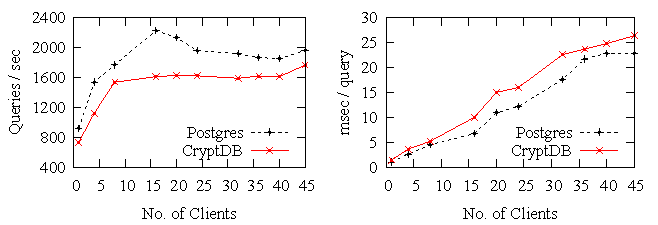
\includegraphics[width=4.3in]{fig/queries.pdf}
\caption{Throughput and latency for TPC-C queries without transactions.}
\label{fig:querytputlat}
\end{minipage}
\hspace{0.3cm}
\begin{minipage}[t]{2.1in}
\centering
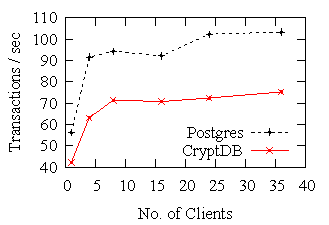
\includegraphics[width=2.05in]{fig/trantput.pdf}
\caption{Throughput of TPC-C transactions.}
\label{fig:trantput}
\end{minipage}
\end{figure*}

% In case of unoptimized \name, client-side
% processing times for each query are increased even further,
% leading to significantly more transaction conflicts and an
% overall throughput reduction of 70\%.

To understand the sources of \name's overhead, we examine the
throughput of individual SQL operators; this analysis is useful
because the mix of operators changes with application.  For each
operator, we collect the corresponding queries from TPC-C, and
measure the latency for those queries running under \name and under
Postgres.  Table~\ref{t:microlat} shows the results.
The proxy encryption time adds an average of 0.34~ms to the query.
The ciphertext caching optimization masks the high latency of queries
requiring $\OPE$ and $\HOM$, as indicated by bold numbers and their
corresponding Proxy$^-$ values.
The DBMS server latencies with and without \name are similar,
suggesting that the expansion of data at the server caused by encryption has a small
impact.
End-to-end, \name with the caching optimization adds
0.64~ms of latency to each query.

Figure~\ref{fig:microtput} shows the throughput for the same mix of
queries for Postgres, \name, and a strawman design that performs each
query by first decrypting the data using a UDF, performing the query,
and re-encrypting the result (if updating the row).  In all cases
except for insert, the strawman performs significantly worse than
\name, since the DBMS cannot use an index to satisfy WHERE clauses. It
is indeed an unexpected fact that the higher security of \name{} over
the strawman in fact also brings better performance. For six SQL
operators (Select equality, Select join, Select range, Delete, Insert,
and Update set), the throughput overhead of \name is negligible
compared to Postgres.  These six constitute most of the queries for
TPC-C, and likely for many other applications.  Homomorphic
operations, such as Select sum and Update increment, incur a
significant overhead with \name, due to the server-side cost of
homomorphically multiplying large cryptographic numbers instead of
adding 32-bit integers.





Adjustable query-based encryption involves decrypting columns to lower
onion levels.  Fortunately, such decryption is fast, and only needs to be
performed once per column for the lifetime of the system.\footnote{One
exception is if the administrator wants to periodically re-encrypt to
increase the security level.}  Removing a layer of $\RND$ requires AES
decryption, which a commodity machine can perform at $\sim$500~MBytes/s.
Thus, removing an onion layer is bottlenecked by the speed at which the
DBMS server can copy a column from disk.

%; the decryption speed
%is negligible in comparison.
% with disk read and write bandwidth.

\subsubsection{Multi-User Web Applications}
\label{s:evalapps}

To evaluate the impact of \name{} on application performance, we
measure the throughput of phpBB for a workload of 30 parallel clients
continuously issuing HTTP requests to browse the forum, write and read
posts, write and read private messages, etc.  We pre-populate forums
and user mailboxes with initial messages.  Figure~\ref{fig:appstput}
shows the throughput of phpBB in four configurations, running on a
single server with MySQL as the DBMS: (1) MySQL, (2) MySQL with the
proxy performing only query parsing, (3) \name with half of phpBB's
sensitive fields encrypted, and (4) \name with all sensitive fields
encrypted.  The results show that phpBB incurs a user-visible
throughput loss of 13\%.  80\% of this loss is from parsing SQL
queries in \name's proxy; an optimized parser would reduce this
overhead.  Finally, the difference between encrypting all the fields
versus half of them is small, indicating that cryptographic operations
are not a problematic bottleneck.

\begin{table}[t]
\small
\begin{tabular}{@{}c|ccccc@{}}
\bf DB & 	\bf Login & 	\bf R post & 	\bf W post & 	\bf R msg & 	\bf W msg \\
\hline
MySQL &			105~ms  & 	85~ms 	&	238~ms	&	107~ms	&	389~ms \\
\name &			183~ms	 &	133~ms	& 	319~ms	&	166~ms	&	481~ms \\
\end{tabular}
\caption{Latency for HTTP requests that heavily use encrypted
    fields in phpBB for MySQL and \name. R and W stand for read and write.}
\label{fig:latencyphpbb}
\end{table}

%To evaluate the latency impact of \name on a real application,
Table~\ref{fig:latencyphpbb} shows the end-to-end latency for
5 types of phpBB requests.  We see that login is slowed down by 78~ms
because \name{} loads keys from the DBMS on login.  Most of the other
latency increases are due to \name's proxy.  Fortunately, the total
increase is small.

\begin{table}[t!]
\centering
\footnotesize
\begin{tabular}{@{}l@{}r|c|c|c@{~}|@{}c@{}}
\multicolumn{2}{l|}{\multirow{2}{*}{\bf Query (\& scheme)}} & \multicolumn{3}{c@{}|}{\bf \name} & \small{\bf Postgres} \\
\cline{3-6}
& & \small{\bf Server} & \small{\bf Proxy} & \small{\bf Proxy$^-$} & \small{\bf Server} \\
\hline
Select by = & ($\DET$) &   0.43~ms    &  0.10~ms   &                 0.10~ms   &  0.41~ms  \\    
Select join & ($\JOIN$)   &   0.72~ms    &   0.27~ms    &           0.27~ms       &  0.63~ms   \\          
Select range & ($\OPE$)  &   1.2~ms    &    \textbf{0.40~ms}     &             58.2~ms    &  0.99~ms   \\       
Select sum & ($\HOM$)     &   8.8~ms    &    0.18~ms   &           0.18~ms   &  0.46~ms   \\
Delete     &  &   1.1~ms    &      0.15~ms   &           0.14~ms       &  1.1~ms   \\                
Insert       & &   1.0~ms    &     \textbf{0.34~ms}   &           18.6~ms    &  0.99~ms   \\                                  
Update set   &  &   1.2~ms    &     0.17~ms   &          0.17~ms   &  1.1~ms   \\                                  
Update incr & ($\HOM$)    &   2.0~ms     &  \textbf{0.71~ms} &         17.7~ms       &   1.8~ms   \\                         
\hline 
Overall   &   &       1.4~ms         &  \textbf{0.34~ms}  &         7.3~ms        &  1.1~ms   \\

\end{tabular}
\caption{Latency for SQL operators.  Proxy is
  the encryption latency for \name{}; ``Proxy$^-$'' is the encryption
  latency without using encryption tables (\S\ref{ss:optimize}).
  Bold numbers show where the caching optimization helps.
  For each operator, we show the predominant encryption scheme
  used. The ``Overall'' row is the average  latency over the mix of
  TPC-C queries. 
  ``Update set'' is an update where the fields are set to a
  constant, and ``Update incr'' is an update 
  where the fields are incremented.}
\label{t:microlat}
\end{table}

\begin{figure}[t!] 
\centering
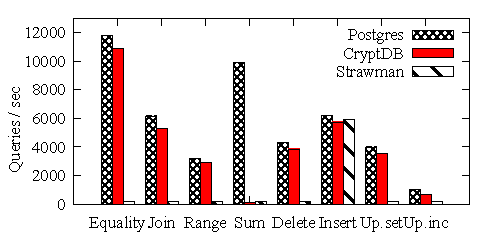
\includegraphics[width=3.1in]{fig/microbars.pdf} 
\caption{Throughput of the SQL operators from Table~\ref{t:microlat}
  running under \name and Postgres. The numbers on top of the bars
  show the throughput reduction with \name{} for that operator. ``Up. inc" stands for update with increment and ``up. set'' for update set.}
\label{fig:microtput}
\end{figure}


\subsubsection{Storage}

The storage overhead of \name can come from two parts: the proxy
and the DBMS\@.
%The proxy stores only the original schema.
The memory footprint of the \name{} proxy process is
18.5~MBytes in our experiments.
Caching the ciphertext of the 100,000 most common values consumes
$<$1 MByte for $\OPE$ and $\sim$12 MBytes for $\HOM$.  On the DBMS
server, for TPC-C, \name{} increased the database size by 4.5$\times$
due to cryptographic expansion of certain integer fields, all fields being encrypted and most of them being integers. In fact, strings and
binary data remain roughly the same size. Consequently,
for phpBB, \name{} increases server storage by 42\%, caused largely
by the public keys of principals (users, groups and messages) and the
$\HOM$ onion for encrypted integer fields.
As the number of posts in a forum grows, the amortized storage overhead
decreases because no new principals are added.

% At the DB server, \name increases the size of the database due to
% onion encryption and tables of principal keys.  For TPC-C, the
% database size using Postgres was 135~MB and with \name, it was
% 619~MB, amounting to 4.5 times increase. This is mostly because of
% aggregates which are large cryptographic numbers, without which it is
% a three fold increase.  Since disk space is relatively cheap, we do
% not consider increased storage cost to be a significant barrier to
% adoption of \name.

%Moreover, there is virtually no expansion for large data items such as
%long strings or binaries.  Therefore, a database storing large text
%or binaries (e.g., photos) will have almost no storage overheads.



\begin{figure}[t]
\centering
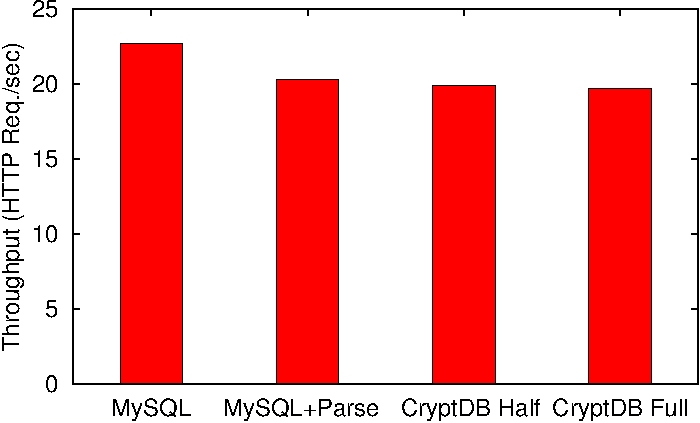
\includegraphics[width=2.3in]{fig/tputbars.pdf} 
\caption{Throughput comparison for phpBB\@. ``MySQL'' denotes phpBB
running directly on MySQL, ``MySQL+Parse'' includes the parsing cost
of \name{} with cryptography and key management removed, ``\name Half''
shows the whole \name{} with half the annotations, and ``\name{} Full''
is the end-to-end system with all sensitive fields annotated.  Most
HTTP requests involved tens of SQL queries each.  Percentages indicate
throughput reduction relative to MySQL\@.}

\label{fig:appstput}
\end{figure}


% must eval adjustable sec!!




